%# -*- coding: utf-8-unix -*-
%%==================================================
\chapter{相对论基础}

本讲义的授课主题,是\gw\DA,共分为两部分,\emph{\gw}与\emph{\DA}。
如果脱离了\gw 的物理图景,而直接空谈\DA,未免空中楼阁。
而在另一方面,引力波又是Einstein广义相对论的直接理论预言,因此,引力波的理论描述,无法跳脱广义相对论的框架。

\begin{figure}[htp]
\centering
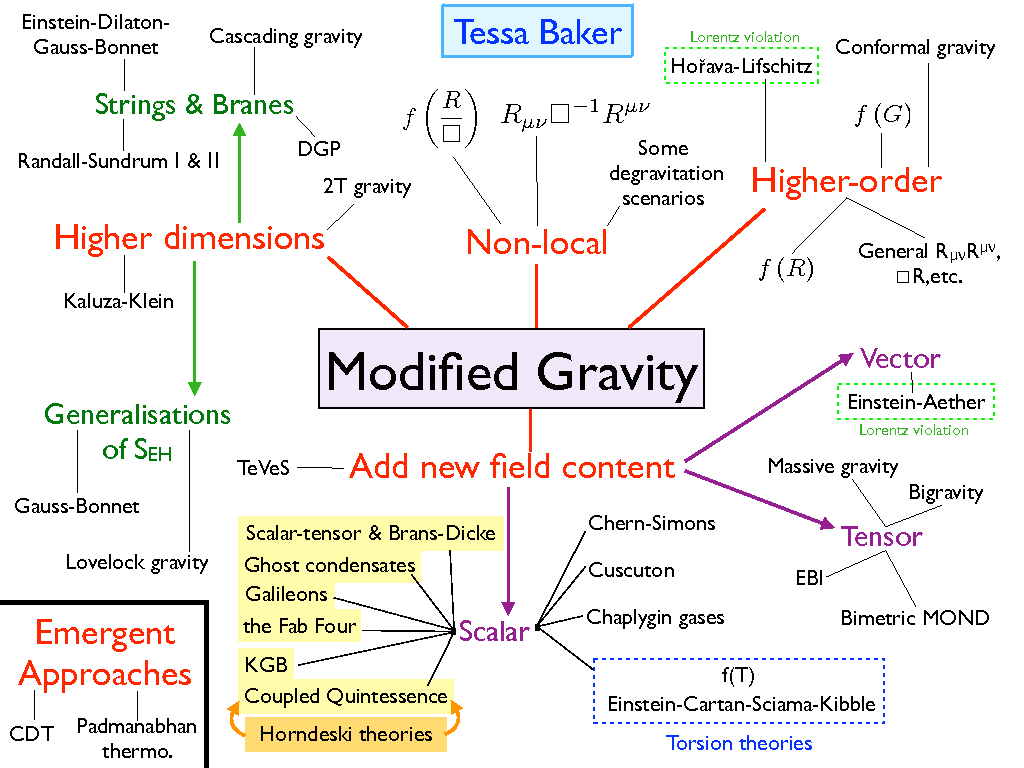
\includegraphics[width=0.7\textwidth]{ModifiedGravity.png}
\bicaption{修改引力理论}
  {Theories of modified gravity. Credit: http://www.cgc-yzu.cn/Upload/research/MG-20240317524.png}
\label{fig:ModGrav}
\end{figure}

从Einstein至今,引力理论已经有了长足的发展,如图\ref{fig:ModGrav}所示,仅基于\GR 基础上发展起来的修改引力理论就已不计其数。
由于和量子力学原理的深刻矛盾,有理由认为Einstein决定论性的的\GR 在某个地方一定背离了引力的物理本质。
然而,时至今日,Einstein昔日基于\GR 所作出的诸多预言,一一被实验所验证;所有可靠的实验检验下,\GR 均可以给出解释——而它通常是最简洁的那个理论。
因此,即使将来的实验证明了\GR 与引力的物理本质之间的偏离,对\GR 的理解依然有着重要的意义。

\section{相对性原理(Principle of relativity)}

\subsection{Galilean相对论}
虽然在20世纪,相对论一次专指Einstein的理论,但是相对性原理(Principle of relativity)的思想在Newtonian力学中就有体现:两个服从Newtonian力学的、相对均匀运动的惯性参考系,无法通过在内部展开的力学实验进行区分。
这一思想一般认为是Galileo在《关于Ptolemaic和 Copernican两大世界体系的对话》中首先提出的\cite{Fang2012blog}:
\begin{myprop}{}{}
把你和一些朋友关在一条大船的甲板下的主舱里,让你们带着几支苍蝇、蝴蝶和其他小飞虫,舱内放一支大碗,其中有几条鱼,然后,挂上一个水瓶,让水一滴一滴地滴到下面的一个宽口罐里。船停着不动时,你留神观察,小虫都以等速向舱内各方向飞行,鱼向各方向随便游动,水滴滴进下面的罐中。你把任何东西扔给你的朋友时,只要距离相等,向这一方向也不比向另一方向更多用力。你的双脚齐跳,无论向哪个方向跳过的距离都相等。当你仔细观察这些事情之后,再使船以任何速度前进,只要运动是均匀的,也不忽左忽右地摆动,你将发现,所有上述现象都没有丝毫变化,你无法从任何一个现象来确定,船是在运动还是在停着不动。即使船运动得相当快,在跳跃时,你也将和以前一样,你跳向船尾也不会比跳向船头更省力。
\end{myprop}
在Galilean相对性原理表明的这个表述中,日常生活中涉及到的物理学性质,在地球坐标系下(船停着不动)和船的坐标系下(船在运动)没有任何区别。

用公式来表述的话,则可以设立两个坐标系,亦即“静止的”地球坐标系S(t,x,y,z)和“运动的”船坐标系S'(t',x',y',z')。
不妨令$t=t'=0$时,两个坐标系重合,且船以速度v沿x方向移动,则有
\begin{equation}
\begin{array}{r@{}l}
t' &{}= t \\
x' &{}= x-vt\\
y' &{}= y \\
z' &{}= z 
\end{array}\label{eq:galileo}
\end{equation}
这种变换通常被称为Galileo变换。

实际上,这种朴素的相对论性原理是非常直观的,在《尚书纬·考灵曜(y{\` a}o)》中,就有文字表达了相当类似的想法:
\begin{myprop}{}{}
地恒动不止,而人不知,如坐闭牖(y{\v o}u)舟中,舟行而人不觉也。
\end{myprop}

\subsection{Maxwell方程组}
通过对电与磁的性质的研究,Maxwell总结了著名的方程组,用以描述电磁场的一般性质。
在真空中,可以记为
\begin{equation}
\begin{array}{r@{}l}
\nabla \cdot \mathbf {E} &{}= {\frac {\rho }{\varepsilon _{0}}}\\
\nabla \cdot \mathbf {B} &{}= 0\\
\nabla \times \mathbf {E}&{}=-{\frac {\partial \mathbf {B} }{\partial t}}\\
\nabla \times \mathbf {B}&{}=\mu _{0}\left(\mathbf {J} +\varepsilon _{0}{\frac {\partial \mathbf {E} }{\partial t}}\right)
\end{array}\label{eq:maxwell}
\end{equation}
其中$\varepsilon_0$为真空电容率,$\mu_0$为真空磁导率。

Maxwell注意到,通过Maxwell方程组,可以推导出,
\begin{equation}
\nabla ^2 \mathbf {B} - \varepsilon_{0} \mu_0 \frac {\partial^2 \mathbf {B} }{\partial^2 t}= 0
\end{equation}
不难看出,电磁场的变化以波动形式传播,其速度$c$取决于:
\begin{equation}
c^2 = \frac{1}{\varepsilon_0 \mu_0} \end{equation} 从数值上,$c$的取值与当时已经从实验上测得的光速极为接近,这使得他大胆假设:光就是一种电磁波。

然而,Maxwell方程组与Galileo变换是不自洽的。
考虑在运动的船S'上进行电磁学测量,根据Galileo变换,电磁场的传播方程变为

\begin{equation}
c^2\nabla^2 \textbf B = \frac{\partial^2 \textbf B}{\partial t^2} + (\textbf v \cdot \nabla)^2 \textbf B - 2 \textbf v \cdot \nabla \left(\frac{\partial \textbf B}{\partial t}\right)
\end{equation}
